\documentclass[xcolor=dvipsnames, aspectratio=169, 10pt]{beamer}
\usepackage[T1]{fontenc}

\usepackage{amsmath, amsfonts, amsthm, amssymb}

\usepackage[mathrm=sym, mathbf=sym]{unicode-math}
\setmathfont{Lete Sans Math}

\AtBeginDocument{%
  \let\mathbb\relax
  \DeclareMathAlphabet{\mathbb}{U}{msb}{m}{n}%
}

\usepackage{graphicx}
\usepackage{float}
\usepackage{bookmark}
\usepackage{enumitem}
\usepackage{tabularray}
\usepackage{animate}

\usepackage{tikz}
\usetikzlibrary{intersections, angles, calc, positioning}

\definecolor{softyellow}{RGB}{252, 222, 165}
\definecolor{tangerine}{RGB}{249, 163, 13}
\definecolor{bgg}{HTML}{fafafa}
\definecolor{bbg}{HTML}{23373b}
\definecolor{orang}{HTML}{eb811b}

\definecolor{backgroundnew}{HTML}{ffebc9}
\setbeamercolor{background canvas}{bg=backgroundnew}
\setbeamercolor{frametitle}{fg=tangerine!90!black}


\usepackage{polyglossia}
\setdefaultlanguage{portuguese}

\usepackage{cancel}

\usepackage{csquotes}
\usepackage[backend=biber, doi=false]{biblatex}
\addbibresource{bibliography.bib}

\newcommand{\medcup}{\mathsf{U}}
\newcommand{\m}{\text{-}}

\newcommand{\bN}{\mathbb{N}}
\newcommand{\bZ}{\mathbb{Z}}
\newcommand{\bQ}{\mathbb{Q}}
\newcommand{\bR}{\mathbb{R}}
\newcommand{\bC}{\mathbb{C}}
\newcommand{\bK}{\mathbb{K}}

\newcommand{\bu}{\mathbf{u}}
\newcommand{\bv}{\mathbf{v}}
\newcommand{\bX}{\mathbf{X}}
\newcommand{\BQ}{\mathbf{Q}}

\newcommand{\cA}{\mathcal{A}}
\newcommand{\cB}{\mathcal{B}}
\newcommand{\cC}{\mathcal{C}}
\newcommand{\cF}{\mathcal{F}}
\newcommand{\cM}{\mathcal{M}}
\newcommand{\cH}{\mathcal{H}}
\newcommand{\cL}{\mathcal{L}}
\newcommand{\cT}{\mathcal{T}}
\newcommand{\cP}{\mathcal{P}}
\newcommand{\cW}{\mathcal{W}}

\newcommand{\supp}{\mathrm{supp}\,}
\newcommand{\esssup}{\mathrm{ess\,sup}\,}
\newcommand{\loc}{\mathrm{loc}}
\newcommand{\sgn}{\mathrm{sgn}}

\newcommand{\doublehookrightarrow}{\;\substack{\hookrightarrow \\ \hookrightarrow}\;}

\newcommand{\sfrac}[2]{{}^{#1}\!\!/\!_{#2}}
\newcommand{\sint}{-\!\!\!\!\!\!\int}

\setbeamertemplate{frametitle}
{%
  \vskip1ex
  \begin{centering}
    \insertframetitle
  \end{centering}
  \vskip1ex
}


\title{Decaimentos das Soluções de Leray e um Problema de
Dirichlet via Espaços de Sobolev}
\author{Bruno Sant'Anna Donato de Moura}
\date{20 de junho de 2025}
\institute{Universidade Federal de Sergipe\\Departamento de Matemática}

% \usetheme[progressbar=foot, block=fill]{metropolis} % https://linorg.usp.br/CTAN/macros/latex/contrib/beamer-contrib/themes/metropolis/doc/metropolistheme.pdf

\setmainfont{Lato Semibold}
\setsansfont{Lato Semibold}
\setmonofont{Iosevka Custom Semibold}
 

\begin{document}
\maketitle

\begin{frame}
    \begin{center}
        \includegraphics[height=4cm]{../sobolev.jpg} \hspace{5mm} 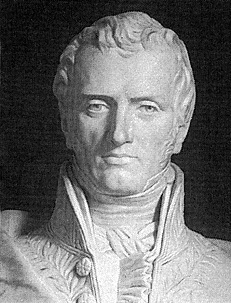
\includegraphics[height=4cm]{../Claude-Louis_Navier.jpg} \hspace{5mm} 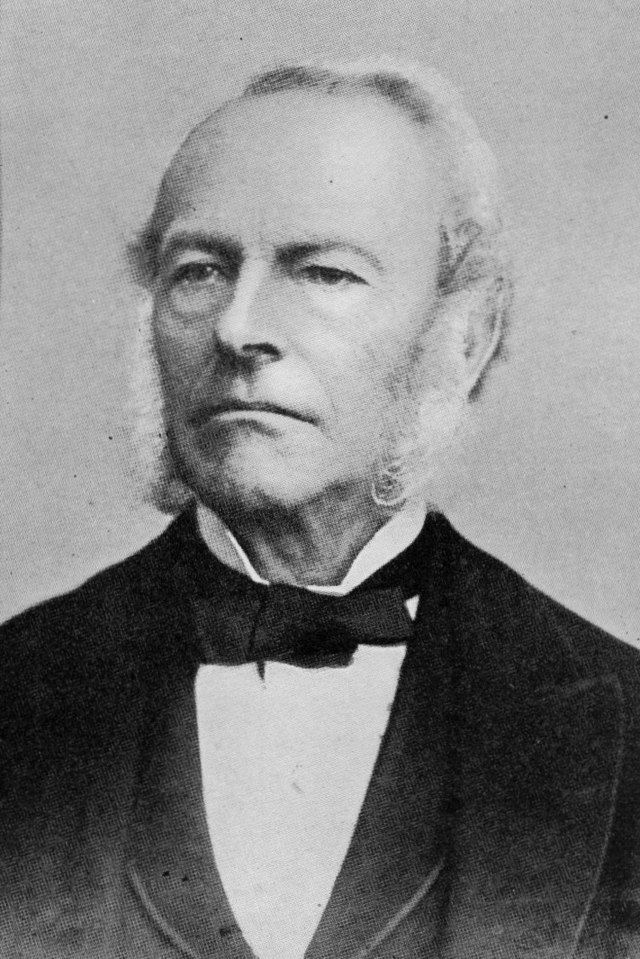
\includegraphics[height=4cm]{../SS-stokes.jpg}
    \end{center}
\end{frame}
\begin{frame}
    \begin{center}
        \bfseries\huge Espaços de Sobolev
    \end{center}
\end{frame}
\begin{frame}
    \frametitle{Motivação}
    Considere o seguinte problema
    \begin{equation} \label{eq:dirichlet}
        \begin{aligned}
            -\Delta u + u &= f, \text{ em } \Omega;\\
            u &= 0, \text{ sobre } \partial\Omega,
        \end{aligned}
    \end{equation}
    onde $\Omega \subseteq \bR^n$ é um aberto limitado. \pause
    Uma solução clássica para o problema acima é uma função $u \in \cC^2(\Omega)$ satisfazendo (\ref{eq:dirichlet}). \pause
    Por outro lado, multiplicando ambos os lados da primeira equação em (\ref{eq:dirichlet}) por uma função $\phi \in \cC^{\infty}_C(\Omega)$ e integrando sobre $\Omega$, obtemos
    \[
        \int_{\mathcal U} - \phi \Delta u \,dx + \int_{\mathcal U} u \phi \,dx = \int_{\mathcal U} f \phi \,dx. \pause
    \]
    Note que, utlizando integração por partes, a primeira integral acima pode ser reescrita como
    \[
        \int_{\Omega} -\phi \Delta u \,dx = -\sum_{i=1}^n \int_{\Omega} \phi \frac{\partial^2 u}{\partial x_i^2} \,dx = -\sum_{i=1}^n \left( \int_{\partial\Omega} \phi \frac{\partial u}{\partial x_i} \nu_i \,dS - \int_{\Omega} \frac{\partial \phi}{\partial x_i} \frac{\partial u}{\partial x_i} \,dx\right).
    \]
\end{frame}
\begin{frame}
    Mas, como $\phi$ se anula sobre $\partial \Omega$, inferimos que
    \[
        \int_{\Omega} -\phi \Delta u \,dx = \sum_{i=1}^n \int_{\Omega} \frac{\partial \phi}{\partial x_i} \frac{\partial u}{\partial x_i} \,dx = \int_{\Omega} \nabla u \cdot \nabla \phi \,dx. \pause
    \]
    Dito isso, dizemos que $u$ é uma solução fraca do problema de Dirichlet se
    \begin{equation} \label{eq:sol-fraca-dirichlet}
        \int_{\Omega} \nabla u \cdot \nabla \phi \,dx + \int_{\Omega} u\phi \,dx = \int_{\Omega} f \phi \,dx,
    \end{equation}
    para toda função $\phi \in \cC^{\infty}_C(\Omega)$. \pause
    Observe agora que, não precisamos mais que $u$ seja de classe $\cC^2$ já que a segunda derivada de $u$ não é utilizada em (\ref{eq:sol-fraca-dirichlet}). Na verdade, não precisamos nem que $u$ seja contínua, apenas integrável em $\Omega$.
\end{frame}

\begin{frame}
    \frametitle{Derivada fraca}
    Nosso primeiro objetivo é generalizar a definição de derivada para funções que não são diferenciáveis no sentido usual. \pause
    Inicialmente, considere $u : \Omega \subseteq \bR^n \to \bR$ uma função de classe $\cC^1$ e $\phi$ uma função teste, utilizando integração por partes podemos escrever
    \[
        \int_{\Omega} u \frac{\partial \phi}{\partial x_i} \,dx = \int_{\partial \Omega} u \phi \nu_i \,dS - \int_{\Omega} \phi \frac{\partial u}{\partial x_i} \,dx,
    \]
    para todo $i = 1,\dots,n$. \pause
    Como $\phi$ tem suporte compacto em um aberto $\Omega$, segue que $\phi \equiv 0$ sobre $\partial \Omega$. Portanto, a expressão acima se torna
    \begin{equation} \label{eq:derivada-fraca-xi}
        \int_{\Omega} u \frac{\partial \phi}{\partial x_i} \,dx = -\int_{\Omega} \phi \frac{\partial u}{\partial x_i} \,dx,
    \end{equation}
    para todo $i = 1,\dots,n$.
\end{frame}
\begin{frame}
    Se agora considerarmos $u \in \cC^k(\Omega)$, com $k \in \bN$ e $\alpha = (\alpha_1,\dots,\alpha_n) \in \bN^n$ um multi-índice de ordem $|\alpha| = \alpha_1 + \cdots + \alpha_n = k$, então
    \begin{equation} \label{eq:derivada-fraca}
        \int_{\Omega} u D^{\alpha} \phi \,dx = (-1)^{|\alpha|} \int_{\Omega} \phi D^{\alpha} u \,dx.
    \end{equation}
    Essa expressão é válida, já que
    \[
        D^{\alpha} = \dfrac{\partial^{\alpha_1} }{\partial x_1^{\alpha_1}} \cdots \dfrac{\partial^{\alpha_n} }{\partial x_n^{\alpha_n}} = \dfrac{\partial^{|\alpha|} }{\partial x_1^{\alpha_1} \cdots \partial x_n^{\alpha_n}},
    \]
    e podemos aplicar (\ref{eq:derivada-fraca-xi}) $|\alpha|$ vezes.
\end{frame}
\begin{frame}
    Queremos descobrir se existe uma classe de funções tal que (\ref{eq:derivada-fraca}) ainda é válida, mesmo se $u$ não for de classe de $\cC^k$. \pause
    Note que, o lado esquerdo de (\ref{eq:derivada-fraca}) está bem definido se $u \in \cL^1_{\loc}(\Omega)$. \pause
    O problema é que se $u$ não for necessáriamente de classe $\cC^k$, não existe garantia de que o lado direito de (\ref{eq:derivada-fraca}) está bem definido.
    Para contornar isso, nos perguntamos se existe uma função $v \in \cL^1_{\loc}(\Omega)$ tal que (\ref{eq:derivada-fraca}) é válida quando substituimos $D^{\alpha} u$ por $v$. \pause

    Sendo assim, definimos a $\alpha$-ésima derivada fraca de uma função $u \in \cL^1_{\loc}(\Omega)$ como a função $v \in \cL^1_{\loc}(\Omega)$ (que denotamos por $D^\alpha u$) tal que
    \[
        \int_{\Omega} u D^\alpha \phi \,dx = (-1)^{|\alpha|} \int_{\Omega} \phi D^\alpha u\,dx,
    \]
    para toda função $\phi \in \cC^{\infty}_c(\Omega)$.
\end{frame}
\begin{frame}
    \frametitle{Exemplos}
    \begin{enumerate}[label=\arabic*.]
        \item A função $u : (-1,1) \to \bR$ dada por $u(x) =|x|$ não é diferenciável mas possui deriavada fraca dada por
        \[
            u'(x) = \sgn(x) = \left\{ 
            \begin{array}{rr}
                1, &\!\text{se }\; x > 0;\\
                0, &\!\text{se }\; x = 0;\\
                -1,&\!\text{se }\; x < 0.
            \end{array}
        \right.
        \] \pause
        \item A função $u : (0,2) \to \bR$ dada por
        \[
        u(x) = \left\{
            \begin{array}{rl}
                x, & \!\text{se }\; 0 < x \leqslant 1;\\
                2, & \!\text{se }\; 1 < x < 2,\\
            \end{array}
        \right.
        \]
        não possui derivada fraca. \pause
        \item A função $u : (-1,1) \times (-1,1) \to \bR$ dada por $u(x_1,x_2) = |x_1|^{\frac{1}{2}} + |x_2|^{\frac{1}{2}}$ não é diferenciável mas possui derivadas pariciais fracas dadas por
        \[
            D^{e_i}u(x_1,x_2) = \frac{1}{2} \sgn(x_i) |x_i|^{\frac{1}{2}}.
        \]
    \end{enumerate}
\end{frame}
\begin{frame}
    \frametitle{Espaços de Sobolev}
    \begin{block}{Definição}
        Sejam $\Omega \subseteq \bR^n$ um aberto, $k \in \bN$ e $1 \leqslant p \leqslant \infty$. Definimos o espaço de Sobolev $\cW^{k,p}(\Omega)$ por
        \[
            \cW^{k,p}(\Omega) = \{u \in \cL^p(\Omega) \,; D^\alpha u \in \cL^p(\Omega), \text{ para todo multi-índice $\alpha$ com } |\alpha| \leqslant k\},
        \]
        onde $D^\alpha u$ é a derivada fraca de $u$
    \end{block} \pause
    \begin{block}{Teorema}
        $(\cW^{k,p}(\Omega), \Vert \cdot \Vert_{\cW^{k,p}(\Omega)})$, com $1 \leqslant p \leqslant \infty$ é um espaço de Banach, onde
        \[
            \Vert u \Vert_{\cW^{k,p}(\Omega)} = \left( \sum_{|\alpha| \leqslant k} \Vert D^\alpha u \Vert_{\cL^p(\Omega)}^p \right)^{\frac{1}{p}},
        \]
        se $1 \leqslant p < \infty$ e
        \[
            \Vert u \Vert_{\cW^{k,\infty}(\Omega)} = \sum_{|\alpha| \leqslant k} \Vert D^\alpha u  \Vert_{\cL^\infty(\Omega)}.
        \]
    \end{block}
\end{frame}
\begin{frame}
    \frametitle{Observações}
    \begin{enumerate}[label=\arabic*.]
        \item Se $p = 2$ denotamos o espaço de Sobolev $\cW^{k,2}(\Omega)$ por $H^k(\Omega)$ pelo fato de ser um espaço de Hilbert, com seu produto interno dado por
        \[
            \left\langle u, v \right\rangle _{H^k(\Omega)} = \sum_{|\alpha| \leqslant k} \int_{\Omega} D^\alpha u \, D^\alpha v \,dx
        \] \pause
        \item Dizemos que uma sequência de funções $(u_n) \subseteq \cW^{k,p}(\Omega)$ converge uma função $u$ em $\cW^{k,p}(\Omega)$ se
        \[
            \Vert u_n - u \Vert_{\cW^{k,p}(\Omega)} \to 0,
        \]
        quando $n \to \infty$. \pause
        \item O espaço $\cW^{k,p}_0(\Omega)$ ($H^k_0(\Omega)$ se $p =2$) é definido como o fecho de $\cC^{\infty}_c(\Omega)$ em $\cW^{k,p}(\Omega)$. Isto é equivalente a dizer que dada uma função $u$ em $\cW^{k,p}_0(\Omega)$ existe uma sequência de funções em $\cC^{\infty}_c(\Omega)$ que converge para $u$ em $\cW^{k,p}(\Omega)$.
    \end{enumerate}
\end{frame}
\begin{frame}
    \frametitle{Propriedades da derivada fraca}
    \begin{enumerate}[label=\arabic*.]
        \item \textbf{(Unicidade)} Se $v$ e $\tilde v$ são derivadas fracas de uma função $u$ então $v = \tilde v$ qtp. \pause
        \item \textbf{(Linearidade)} Se $u, v \in \cW^{k,p}(\Omega)$ e $\lambda \in \bR$, então $\lambda u + v \in \cW^{k,p}(\Omega)$ e
        \[
            D^\alpha(\lambda u + v) = \lambda D^\alpha u + D^\alpha v.
        \] \pause
        \item \textbf{(Regra de Leibniz)} Se $u \in \cW^{k,p}(\Omega)$ e $\eta \in \cC^{\infty}_c(\Omega)$, então $\eta u \in \cW^{k,p}(\Omega)$ e
        \begin{equation} \label{eq:regra-de-leibniz}
            D^\alpha (\eta u) = \sum_{\sigma \leqslant \alpha} \binom{\alpha}{\sigma} D^{\sigma} \eta D^{\alpha - \sigma} u,
        \end{equation}
        onde
        \[
            \binom{\alpha}{\sigma} = \frac{\alpha!}{\sigma!(\alpha - \sigma)!}, \quad \alpha! = \alpha_1!\cdots \alpha_n!
        \]
        e $\sigma \leqslant \alpha$ significa $\sigma_j \leqslant \alpha_j$, para todo $j = 1,\dots,n$.
    \end{enumerate}
\end{frame}
\begin{frame}
    \frametitle{Aproximações}
    A definição de derivada fraca, em muitos casos, não é suficiente para mostrar propriedades mais
    profundas dos espaços de Sobolev. Uma forma de contornar esse problema é procurando formas
    de aproximar em $\cW^{k,p}$ por uma sequência de funções suaves. Esse processo é conhecido como
    molificação ou regularização e é feito por meio de uma convolução da função a ser aproximada e
    uma função especial chamada função molificadora \pause

    Um exemplo de função molificadora é
    \begin{equation} \label{eq:molificador-friedrich}
        \eta(x) =
        \left\{
            \begin{array}{lr}
                c \exp \left( \frac{1}{|x|^2 - 1} \right), &\! \text{se }\; |x| < 1;\\
                0, &\!\text{se }\; |x| \geqslant 1,
            \end{array}
        \right.
    \end{equation}
\end{frame}
\begin{frame}
    Dada uma função molificadora, para cada $\varepsilon > 0$, definimos $\eta_\varepsilon$ dada por
    \[
        \eta_\varepsilon(x) = \frac{1}{\varepsilon^n} \eta \left( \frac{x}{\varepsilon} \right).
    \]
    Essa aplicação será utilizada para realizar as convoluções que aproximam as funções em $\cW^{k,p}$.
    Se $u$ é uma função localmente integrável, definimos a \textbf{molificação} de $u$ por $u^\varepsilon = \eta_\varepsilon * u$, isto é
    \[
        u^\varepsilon(x) = \int_\Omega \eta_\varepsilon(x-y) u(y) = \int_{B[0,\varepsilon]} \eta_\varepsilon(y) u(x-y) \,dy,
    \]
    para todo $x \in \bR^n$.
\end{frame}
\begin{frame}
    \begin{center}
        \begin{tikzpicture}[scale=0.9]
            \begin{scope}[shift={(-4,0)}, scale=0.8]
                \draw[black!30] (-4,-4) grid (4,4);
                \draw[thick, black!60, -stealth] (-4,0) to (4,0); 
                \draw[thick, black!60, -stealth] (0,-4) to (0,4); 
                \draw[domain=-0.9999:0.9999, variable=\x, samples=50, smooth, ultra thick, tangerine!90!black] plot ({\x}, {2.257 * exp(-1 / (1 - (\x * \x)))});
                \draw[ultra thick, tangerine!90!black] (-1,0) -- (-3,0);
                \draw[ultra thick, tangerine!90!black] (1,0) -- (3,0);
            \end{scope}

            \begin{scope}[shift={(4,0)}, scale=0.8]
                \draw[black!30] (-4,-4) grid (4,4);
                \draw[thick, black!60, -stealth] (-4,0) to (4,0); 
                \draw[thick, black!60, -stealth] (0,-4) to (0,4); 
                \draw[domain=-0.299:0.299, variable=\x, samples=50, smooth, ultra thick, tangerine!90!black] plot ({\x}, {(1/0.3) * 2.257 * exp(-1 / (1 - ((\x / 0.3) * (\x / 0.3))))});
                \draw[ultra thick, tangerine!90!black] (-0.3,0) -- (-3,0);
                \draw[ultra thick, tangerine!90!black] (0.3,0) -- (3,0);
            \end{scope}
        \end{tikzpicture}
    \end{center}
\end{frame}
\begin{frame}
    \begin{center}
        \includegraphics[width=0.43\textwidth]{../2η.pdf}
        \hspace{10mm}
        \includegraphics[width=0.43\textwidth]{../2ηε.pdf}
    \end{center}
\end{frame}
\begin{frame}
    \frametitle{Exemplos}
    \begin{center}
        \begin{tikzpicture}
    \draw[thin, black!30] (-4,-4) grid[step=1] (4,4);
    \draw[thick, black!60, -stealth] (-4,0) to (4,0); 
    \draw[thick, black!60, -stealth] (0,-4) to (0,4);

    \node[align=left, anchor=south west] at (-3.9,-3.9) {$\textcolor{tangerine!90!black}{\blacksquare\!\blacksquare \;\; \varepsilon =1}$ \\ $\textcolor{BrickRed}{\blacksquare\!\blacksquare \;\; \varepsilon = 0.5}$ \\ $\textcolor{orange}{\blacksquare\!\blacksquare \;\; \varepsilon = 0.25}$};
    
    \coordinate (01-1) at (-3.000, 3.000);
    \coordinate (02-1) at (-2.940, 2.940);
    \coordinate (03-1) at (-2.880, 2.880);
    \coordinate (04-1) at (-2.817, 2.817);
    \coordinate (05-1) at (-2.757, 2.757);
    \coordinate (06-1) at (-2.697, 2.697);
    \coordinate (07-1) at (-2.637, 2.637);
    \coordinate (08-1) at (-2.577, 2.577);
    \coordinate (09-1) at (-2.514, 2.517);
    \coordinate (10-1) at (-2.454, 2.454);
    \coordinate (11-1) at (-2.394, 2.394);
    \coordinate (12-1) at (-2.334, 2.337);
    \coordinate (13-1) at (-2.274, 2.277);
    \coordinate (14-1) at (-2.211, 2.217);
    \coordinate (15-1) at (-2.151, 2.160);
    \coordinate (16-1) at (-2.091, 2.103);
    \coordinate (17-1) at (-2.031, 2.046);
    \coordinate (18-1) at (-1.971, 1.992);
    \coordinate (19-1) at (-1.908, 1.935);
    \coordinate (20-1) at (-1.848, 1.884);
    \coordinate (21-1) at (-1.788, 1.830);
    \coordinate (22-1) at (-1.728, 1.779);
    \coordinate (23-1) at (-1.668, 1.728);
    \coordinate (24-1) at (-1.605, 1.680);
    \coordinate (25-1) at (-1.545, 1.632);
    \coordinate (26-1) at (-1.485, 1.587);
    \coordinate (27-1) at (-1.425, 1.542);
    \coordinate (28-1) at (-1.365, 1.497);
    \coordinate (29-1) at (-1.302, 1.458);
    \coordinate (30-1) at (-1.242, 1.416);
    \coordinate (31-1) at (-1.182, 1.380);
    \coordinate (32-1) at (-1.122, 1.341);
    \coordinate (33-1) at (-1.062, 1.308);
    \coordinate (34-1) at (-0.999, 1.275);
    \coordinate (35-1) at (-0.939, 1.242);
    \coordinate (36-1) at (-0.879, 1.215);
    \coordinate (37-1) at (-0.819, 1.185);
    \coordinate (38-1) at (-0.759, 1.161);
    \coordinate (39-1) at (-0.696, 1.137);
    \coordinate (40-1) at (-0.636, 1.113);
    \coordinate (41-1) at (-0.576, 1.095);
    \coordinate (42-1) at (-0.516, 1.077);
    \coordinate (43-1) at (-0.456, 1.059);
    \coordinate (44-1) at (-0.393, 1.047);
    \coordinate (45-1) at (-0.333, 1.035);
    \coordinate (46-1) at (-0.273, 1.023);
    \coordinate (47-1) at (-0.213, 1.017);
    \coordinate (48-1) at (-0.153, 1.011);
    \coordinate (49-1) at (-0.090, 1.005);
    \coordinate (50-1) at (-0.030, 1.005);
    \coordinate (51-1) at (0.030, 1.005);
    \coordinate (52-1) at (0.090, 1.005);
    \coordinate (53-1) at (0.153, 1.011);
    \coordinate (54-1) at (0.213, 1.017);
    \coordinate (55-1) at (0.273, 1.023);
    \coordinate (56-1) at (0.333, 1.035);
    \coordinate (57-1) at (0.393, 1.047);
    \coordinate (58-1) at (0.456, 1.059);
    \coordinate (59-1) at (0.516, 1.077);
    \coordinate (60-1) at (0.576, 1.095);
    \coordinate (61-1) at (0.636, 1.113);
    \coordinate (62-1) at (0.696, 1.137);
    \coordinate (63-1) at (0.759, 1.161);
    \coordinate (64-1) at (0.819, 1.185);
    \coordinate (65-1) at (0.879, 1.215);
    \coordinate (66-1) at (0.939, 1.242);
    \coordinate (67-1) at (0.999, 1.275);
    \coordinate (68-1) at (1.062, 1.308);
    \coordinate (69-1) at (1.122, 1.341);
    \coordinate (70-1) at (1.182, 1.380);
    \coordinate (71-1) at (1.242, 1.416);
    \coordinate (72-1) at (1.302, 1.458);
    \coordinate (73-1) at (1.365, 1.497);
    \coordinate (74-1) at (1.425, 1.542);
    \coordinate (75-1) at (1.485, 1.587);
    \coordinate (76-1) at (1.545, 1.632);
    \coordinate (77-1) at (1.605, 1.680);
    \coordinate (78-1) at (1.668, 1.728);
    \coordinate (79-1) at (1.728, 1.779);
    \coordinate (80-1) at (1.788, 1.830);
    \coordinate (81-1) at (1.848, 1.884);
    \coordinate (82-1) at (1.908, 1.935);
    \coordinate (83-1) at (1.971, 1.992);
    \coordinate (84-1) at (2.031, 2.046);
    \coordinate (85-1) at (2.091, 2.103);
    \coordinate (86-1) at (2.151, 2.160);
    \coordinate (87-1) at (2.211, 2.217);
    \coordinate (88-1) at (2.274, 2.277);
    \coordinate (89-1) at (2.334, 2.337);
    \coordinate (90-1) at (2.394, 2.394);
    \coordinate (91-1) at (2.454, 2.454);
    \coordinate (92-1) at (2.514, 2.517);
    \coordinate (93-1) at (2.577, 2.577);
    \coordinate (94-1) at (2.637, 2.637);
    \coordinate (95-1) at (2.697, 2.697);
    \coordinate (96-1) at (2.757, 2.757);
    \coordinate (97-1) at (2.817, 2.817);
    \coordinate (98-1) at (2.880, 2.880);
    \coordinate (99-1) at (2.940, 2.940);
    \coordinate (00-1) at (3.000, 3.000);

    \coordinate (01-2) at (-3.000, 3.000);
    \coordinate (02-2) at (-2.940, 2.940);
    \coordinate (03-2) at (-2.880, 2.880);
    \coordinate (04-2) at (-2.817, 2.817);
    \coordinate (05-2) at (-2.757, 2.757);
    \coordinate (06-2) at (-2.697, 2.697);
    \coordinate (07-2) at (-2.637, 2.637);
    \coordinate (08-2) at (-2.577, 2.577);
    \coordinate (09-2) at (-2.514, 2.514);
    \coordinate (10-2) at (-2.454, 2.454);
    \coordinate (11-2) at (-2.394, 2.394);
    \coordinate (12-2) at (-2.334, 2.334);
    \coordinate (13-2) at (-2.274, 2.274);
    \coordinate (14-2) at (-2.211, 2.211);
    \coordinate (15-2) at (-2.151, 2.151);
    \coordinate (16-2) at (-2.091, 2.091);
    \coordinate (17-2) at (-2.031, 2.031);
    \coordinate (18-2) at (-1.971, 1.971);
    \coordinate (19-2) at (-1.908, 1.908);
    \coordinate (20-2) at (-1.848, 1.848);
    \coordinate (21-2) at (-1.788, 1.788);
    \coordinate (22-2) at (-1.728, 1.728);
    \coordinate (23-2) at (-1.668, 1.668);
    \coordinate (24-2) at (-1.605, 1.605);
    \coordinate (25-2) at (-1.545, 1.545);
    \coordinate (26-2) at (-1.485, 1.485);
    \coordinate (27-2) at (-1.425, 1.425);
    \coordinate (28-2) at (-1.365, 1.365);
    \coordinate (29-2) at (-1.302, 1.302);
    \coordinate (30-2) at (-1.242, 1.242);
    \coordinate (31-2) at (-1.182, 1.182);
    \coordinate (32-2) at (-1.122, 1.125);
    \coordinate (33-2) at (-1.062, 1.065);
    \coordinate (34-2) at (-0.999, 1.008);
    \coordinate (35-2) at (-0.939, 0.954);
    \coordinate (36-2) at (-0.879, 0.903);
    \coordinate (37-2) at (-0.819, 0.852);
    \coordinate (38-2) at (-0.759, 0.804);
    \coordinate (39-2) at (-0.696, 0.759);
    \coordinate (40-2) at (-0.636, 0.717);
    \coordinate (41-2) at (-0.576, 0.681);
    \coordinate (42-2) at (-0.516, 0.645);
    \coordinate (43-2) at (-0.456, 0.615);
    \coordinate (44-2) at (-0.393, 0.585);
    \coordinate (45-2) at (-0.333, 0.564);
    \coordinate (46-2) at (-0.273, 0.543);
    \coordinate (47-2) at (-0.213, 0.525);
    \coordinate (48-2) at (-0.153, 0.513);
    \coordinate (49-2) at (-0.090, 0.507);
    \coordinate (50-2) at (-0.030, 0.501);
    \coordinate (51-2) at (0.030, 0.501);
    \coordinate (52-2) at (0.090, 0.507);
    \coordinate (53-2) at (0.153, 0.513);
    \coordinate (54-2) at (0.213, 0.525);
    \coordinate (55-2) at (0.273, 0.543);
    \coordinate (56-2) at (0.333, 0.564);
    \coordinate (57-2) at (0.393, 0.585);
    \coordinate (58-2) at (0.456, 0.615);
    \coordinate (59-2) at (0.516, 0.645);
    \coordinate (60-2) at (0.576, 0.681);
    \coordinate (61-2) at (0.636, 0.717);
    \coordinate (62-2) at (0.696, 0.759);
    \coordinate (63-2) at (0.759, 0.804);
    \coordinate (64-2) at (0.819, 0.852);
    \coordinate (65-2) at (0.879, 0.903);
    \coordinate (66-2) at (0.939, 0.954);
    \coordinate (67-2) at (0.999, 1.008);
    \coordinate (68-2) at (1.062, 1.065);
    \coordinate (69-2) at (1.122, 1.125);
    \coordinate (70-2) at (1.182, 1.182);
    \coordinate (71-2) at (1.242, 1.242);
    \coordinate (72-2) at (1.302, 1.302);
    \coordinate (73-2) at (1.365, 1.365);
    \coordinate (74-2) at (1.425, 1.425);
    \coordinate (75-2) at (1.485, 1.485);
    \coordinate (76-2) at (1.545, 1.545);
    \coordinate (77-2) at (1.605, 1.605);
    \coordinate (78-2) at (1.668, 1.668);
    \coordinate (79-2) at (1.728, 1.728);
    \coordinate (80-2) at (1.788, 1.788);
    \coordinate (81-2) at (1.848, 1.848);
    \coordinate (82-2) at (1.908, 1.908);
    \coordinate (83-2) at (1.971, 1.971);
    \coordinate (84-2) at (2.031, 2.031);
    \coordinate (85-2) at (2.091, 2.091);
    \coordinate (86-2) at (2.151, 2.151);
    \coordinate (87-2) at (2.211, 2.211);
    \coordinate (88-2) at (2.274, 2.274);
    \coordinate (89-2) at (2.334, 2.334);
    \coordinate (90-2) at (2.394, 2.394);
    \coordinate (91-2) at (2.454, 2.454);
    \coordinate (92-2) at (2.514, 2.514);
    \coordinate (93-2) at (2.577, 2.577);
    \coordinate (94-2) at (2.637, 2.637);
    \coordinate (95-2) at (2.697, 2.697);
    \coordinate (96-2) at (2.757, 2.757);
    \coordinate (97-2) at (2.817, 2.817);
    \coordinate (98-2) at (2.880, 2.880);
    \coordinate (99-2) at (2.940, 2.940);
    \coordinate (00-2) at (3.000, 3.000);

    \coordinate (01-3) at (-3.000, 3.000);
    \coordinate (02-3) at (-2.940, 2.940);
    \coordinate (03-3) at (-2.880, 2.880);
    \coordinate (04-3) at (-2.817, 2.817);
    \coordinate (05-3) at (-2.757, 2.757);
    \coordinate (06-3) at (-2.697, 2.697);
    \coordinate (07-3) at (-2.637, 2.637);
    \coordinate (08-3) at (-2.577, 2.577);
    \coordinate (09-3) at (-2.514, 2.514);
    \coordinate (10-3) at (-2.454, 2.454);
    \coordinate (11-3) at (-2.394, 2.394);
    \coordinate (12-3) at (-2.334, 2.334);
    \coordinate (13-3) at (-2.274, 2.274);
    \coordinate (14-3) at (-2.211, 2.211);
    \coordinate (15-3) at (-2.151, 2.151);
    \coordinate (16-3) at (-2.091, 2.091);
    \coordinate (17-3) at (-2.031, 2.031);
    \coordinate (18-3) at (-1.971, 1.971);
    \coordinate (19-3) at (-1.908, 1.908);
    \coordinate (20-3) at (-1.848, 1.848);
    \coordinate (21-3) at (-1.788, 1.788);
    \coordinate (22-3) at (-1.728, 1.728);
    \coordinate (23-3) at (-1.668, 1.668);
    \coordinate (24-3) at (-1.605, 1.605);
    \coordinate (25-3) at (-1.545, 1.545);
    \coordinate (26-3) at (-1.485, 1.485);
    \coordinate (27-3) at (-1.425, 1.425);
    \coordinate (28-3) at (-1.365, 1.365);
    \coordinate (29-3) at (-1.302, 1.302);
    \coordinate (30-3) at (-1.242, 1.242);
    \coordinate (31-3) at (-1.182, 1.182);
    \coordinate (32-3) at (-1.122, 1.122);
    \coordinate (33-3) at (-1.062, 1.062);
    \coordinate (34-3) at (-0.999, 0.999);
    \coordinate (35-3) at (-0.939, 0.939);
    \coordinate (36-3) at (-0.879, 0.879);
    \coordinate (37-3) at (-0.819, 0.819);
    \coordinate (38-3) at (-0.759, 0.759);
    \coordinate (39-3) at (-0.696, 0.696);
    \coordinate (40-3) at (-0.636, 0.636);
    \coordinate (41-3) at (-0.576, 0.576);
    \coordinate (42-3) at (-0.516, 0.519);
    \coordinate (43-3) at (-0.456, 0.465);
    \coordinate (44-3) at (-0.393, 0.414);
    \coordinate (45-3) at (-0.333, 0.369);
    \coordinate (46-3) at (-0.273, 0.330);
    \coordinate (47-3) at (-0.213, 0.300);
    \coordinate (48-3) at (-0.153, 0.276);
    \coordinate (49-3) at (-0.090, 0.261);
    \coordinate (50-3) at (-0.030, 0.252);
    \coordinate (51-3) at (0.030, 0.252);
    \coordinate (52-3) at (0.090, 0.261);
    \coordinate (53-3) at (0.153, 0.276);
    \coordinate (54-3) at (0.213, 0.300);
    \coordinate (55-3) at (0.273, 0.330);
    \coordinate (56-3) at (0.333, 0.369);
    \coordinate (57-3) at (0.393, 0.414);
    \coordinate (58-3) at (0.456, 0.465);
    \coordinate (59-3) at (0.516, 0.519);
    \coordinate (60-3) at (0.576, 0.576);
    \coordinate (61-3) at (0.636, 0.636);
    \coordinate (62-3) at (0.696, 0.696);
    \coordinate (63-3) at (0.759, 0.759);
    \coordinate (64-3) at (0.819, 0.819);
    \coordinate (65-3) at (0.879, 0.879);
    \coordinate (66-3) at (0.939, 0.939);
    \coordinate (67-3) at (0.999, 0.999);
    \coordinate (68-3) at (1.062, 1.062);
    \coordinate (69-3) at (1.122, 1.122);
    \coordinate (70-3) at (1.182, 1.182);
    \coordinate (71-3) at (1.242, 1.242);
    \coordinate (72-3) at (1.302, 1.302);
    \coordinate (73-3) at (1.365, 1.365);
    \coordinate (74-3) at (1.425, 1.425);
    \coordinate (75-3) at (1.485, 1.485);
    \coordinate (76-3) at (1.545, 1.545);
    \coordinate (77-3) at (1.605, 1.605);
    \coordinate (78-3) at (1.668, 1.668);
    \coordinate (79-3) at (1.728, 1.728);
    \coordinate (80-3) at (1.788, 1.788);
    \coordinate (81-3) at (1.848, 1.848);
    \coordinate (82-3) at (1.908, 1.908);
    \coordinate (83-3) at (1.971, 1.971);
    \coordinate (84-3) at (2.031, 2.031);
    \coordinate (85-3) at (2.091, 2.091);
    \coordinate (86-3) at (2.151, 2.151);
    \coordinate (87-3) at (2.211, 2.211);
    \coordinate (88-3) at (2.274, 2.274);
    \coordinate (89-3) at (2.334, 2.334);
    \coordinate (90-3) at (2.394, 2.394);
    \coordinate (91-3) at (2.454, 2.454);
    \coordinate (92-3) at (2.514, 2.514);
    \coordinate (93-3) at (2.577, 2.577);
    \coordinate (94-3) at (2.637, 2.637);
    \coordinate (95-3) at (2.697, 2.697);
    \coordinate (96-3) at (2.757, 2.757);
    \coordinate (97-3) at (2.817, 2.817);
    \coordinate (98-3) at (2.880, 2.880);
    \coordinate (99-3) at (2.940, 2.940);
    \coordinate (00-3) at (3.000, 3.000);

    \draw[very thick, dashed] (-3,3) -- (0,0) -- (3,3);

    \draw[very thick, tangerine!90!black] 
       (01-1) -- (02-1) -- (03-1) -- (04-1) -- (05-1) -- (06-1) -- (07-1) -- (08-1) -- (09-1) -- (10-1)
    -- (11-1) -- (12-1) -- (13-1) -- (14-1) -- (15-1) -- (16-1) -- (17-1) -- (18-1) -- (19-1) -- (20-1)
    -- (21-1) -- (22-1) -- (23-1) -- (24-1) -- (25-1) -- (26-1) -- (27-1) -- (28-1) -- (29-1) -- (30-1)
    -- (31-1) -- (32-1) -- (33-1) -- (34-1) -- (35-1) -- (36-1) -- (37-1) -- (38-1) -- (39-1) -- (40-1)
    -- (41-1) -- (42-1) -- (43-1) -- (44-1) -- (45-1) -- (46-1) -- (47-1) -- (48-1) -- (49-1) -- (50-1)
    -- (51-1) -- (52-1) -- (53-1) -- (54-1) -- (55-1) -- (56-1) -- (57-1) -- (58-1) -- (59-1) -- (60-1)
    -- (61-1) -- (62-1) -- (63-1) -- (64-1) -- (65-1) -- (66-1) -- (67-1) -- (68-1) -- (69-1) -- (70-1)
    -- (71-1) -- (72-1) -- (73-1) -- (74-1) -- (75-1) -- (76-1) -- (77-1) -- (78-1) -- (79-1) -- (80-1)
    -- (81-1) -- (82-1) -- (83-1) -- (84-1) -- (85-1) -- (86-1) -- (87-1) -- (88-1) -- (89-1) -- (90-1)
    -- (91-1) -- (92-1) -- (93-1) -- (94-1) -- (95-1) -- (96-1) -- (97-1) -- (98-1) -- (99-1) -- (00-1);

    \draw[very thick, BrickRed] 
       (01-2) -- (02-2) -- (03-2) -- (04-2) -- (05-2) -- (06-2) -- (07-2) -- (08-2) -- (09-2) -- (10-2)
    -- (11-2) -- (12-2) -- (13-2) -- (14-2) -- (15-2) -- (16-2) -- (17-2) -- (18-2) -- (19-2) -- (20-2)
    -- (21-2) -- (22-2) -- (23-2) -- (24-2) -- (25-2) -- (26-2) -- (27-2) -- (28-2) -- (29-2) -- (30-2)
    -- (31-2) -- (32-2) -- (33-2) -- (34-2) -- (35-2) -- (36-2) -- (37-2) -- (38-2) -- (39-2) -- (40-2)
    -- (41-2) -- (42-2) -- (43-2) -- (44-2) -- (45-2) -- (46-2) -- (47-2) -- (48-2) -- (49-2) -- (50-2)
    -- (51-2) -- (52-2) -- (53-2) -- (54-2) -- (55-2) -- (56-2) -- (57-2) -- (58-2) -- (59-2) -- (60-2)
    -- (61-2) -- (62-2) -- (63-2) -- (64-2) -- (65-2) -- (66-2) -- (67-2) -- (68-2) -- (69-2) -- (70-2)
    -- (71-2) -- (72-2) -- (73-2) -- (74-2) -- (75-2) -- (76-2) -- (77-2) -- (78-2) -- (79-2) -- (80-2)
    -- (81-2) -- (82-2) -- (83-2) -- (84-2) -- (85-2) -- (86-2) -- (87-2) -- (88-2) -- (89-2) -- (90-2)
    -- (91-2) -- (92-2) -- (93-2) -- (94-2) -- (95-2) -- (96-2) -- (97-2) -- (98-2) -- (99-2) -- (00-2);

    \draw[very thick, orange] 
       (01-3) -- (02-3) -- (03-3) -- (04-3) -- (05-3) -- (06-3) -- (07-3) -- (08-3) -- (09-3) -- (10-3)
    -- (11-3) -- (12-3) -- (13-3) -- (14-3) -- (15-3) -- (16-3) -- (17-3) -- (18-3) -- (19-3) -- (20-3)
    -- (21-3) -- (22-3) -- (23-3) -- (24-3) -- (25-3) -- (26-3) -- (27-3) -- (28-3) -- (29-3) -- (30-3)
    -- (31-3) -- (32-3) -- (33-3) -- (34-3) -- (35-3) -- (36-3) -- (37-3) -- (38-3) -- (39-3) -- (40-3)
    -- (41-3) -- (42-3) -- (43-3) -- (44-3) -- (45-3) -- (46-3) -- (47-3) -- (48-3) -- (49-3) -- (50-3)
    -- (51-3) -- (52-3) -- (53-3) -- (54-3) -- (55-3) -- (56-3) -- (57-3) -- (58-3) -- (59-3) -- (60-3)
    -- (61-3) -- (62-3) -- (63-3) -- (64-3) -- (65-3) -- (66-3) -- (67-3) -- (68-3) -- (69-3) -- (70-3)
    -- (71-3) -- (72-3) -- (73-3) -- (74-3) -- (75-3) -- (76-3) -- (77-3) -- (78-3) -- (79-3) -- (80-3)
    -- (81-3) -- (82-3) -- (83-3) -- (84-3) -- (85-3) -- (86-3) -- (87-3) -- (88-3) -- (89-3) -- (90-3)
    -- (91-3) -- (92-3) -- (93-3) -- (94-3) -- (95-3) -- (96-3) -- (97-3) -- (98-3) -- (99-3) -- (00-3);
\end{tikzpicture}
\\
        Aproximações suaves da função $|x|$
    \end{center}
\end{frame}
\begin{frame}
    \frametitle{Exemplos}
    \begin{center}
        \includegraphics[width=0.4\columnwidth]{../u.pdf}
        \hspace{10mm}
        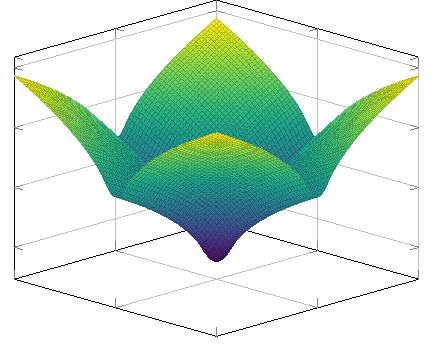
\includegraphics[width=0.4\columnwidth]{../uε2.pdf}\\
        À esquerda, a função $u(x_1,x_2) = |x_1|^{\frac{1}{2}} + |x_2|^{\frac{1}{2}}$ e à direita sua aproximação\\suave $u^\varepsilon$ com $\varepsilon = 0.25$.\\Fonte: Autoral.
    \end{center}
\end{frame}
\begin{frame}
    \frametitle{Resultados}
    \uncover<1>{Nesse capítulo estudamos três resultados}

    \only<1>{
    \begin{block}{Teorema}
        Seja $u \in \cW^{k,p}(\Omega)$, com $1 \leqslant p < \infty$, e defina
        \[
            u^{\varepsilon} = \eta_{\varepsilon} * u \;\text{ em } \Omega_\varepsilon,
        \]
        onde
        \[
            \Omega_\varepsilon = \{ x \in \Omega \,; d(x,\partial\Omega) > \varepsilon\}.
        \]
        Então,
        \begin{enumerate}[leftmargin=*, label=\textbf{(\alph*)}]
            \item $u^\varepsilon \in \cC^{\infty}(\Omega_\varepsilon)$, para cada $\varepsilon > 0$;
            \item $u^\varepsilon \to u$ em $\cW^{k,p}_{\mathrm{loc}}(\Omega)$, quando $\varepsilon \to 0$.
        \end{enumerate}
    \end{block}}

    \only<2>{
    \begin{block}{Teorema}
        Sejam $\Omega$ um aberto limitado e $u \in \cW^{k,p}(\Omega)$, com $1 \leqslant p < \infty$.
        Então, existe uma sequência $(u_n) \subseteq \cC^{\infty}(\Omega) \cap \cW^{k,p}(\Omega)$ tal que
        \[
            u_n \to u \;\text{ em } \cW^{k,p}(\Omega),
        \] 
        quando $n \to \infty$.
    \end{block}}

    \only<3>{
    \begin{block}{Teorema}
        Sejam $\Omega$ um aberto limitado com fronteira de classe $\cC^1$ e $u \in \cW^{k,p}(\Omega)$, com $1 \leqslant p < \infty$.
        Então, existe uma sequência $(u_n) \subseteq \cC^\infty(\overline\Omega)$ tal que
        \[
            u_n \to u \;\text{ em } \cW^{k,p}(\Omega),
        \]
        quando $n \to \infty$.
    \end{block}}
\end{frame}
\begin{frame}
    \frametitle{Extensões}
    Em alguns casos é mais viável trabalhar com funções definidas no espaço Euclidiano inteiro ao invés de funções definida em um aberto específico.
    
    \pause
    Nessa seção estudamos o resultado abaixo
    \begin{block}{Teorema}
         Sejam $\Omega$ um aberto limitado, com fronteira de classe $\cC^1$ e $\Omega'$ um aberto tal que $\Omega \Subset \Omega'$. Então, existe um operador linear limitado $E : \cW^{1,p}(\Omega) \to \cW^{1,p}(\bR ^n)$, com $1 \leqslant p < \infty$, tal que para cada $u \in \cW^{1,p}(\Omega)$, tem-se que
    \begin{enumerate}[leftmargin=*, label=\textbf{(\alph*)}]
        \item $Eu = u$ qtp em $\Omega$;
        \item $\supp Eu \subseteq \Omega'$;
        \item $\Vert Eu \Vert_{\cW^{1,p}(\bR^n)} \leqslant c \Vert u \Vert_{\cW^{1,p}(\Omega)}$, onde a constante $c$ depende apenas de $p$, $\Omega$ e $\Omega'$.
    \end{enumerate}
    \end{block}
\end{frame}
\begin{frame}
    \frametitle{Traços}

    Em alguns casos, no estudo de equações diferenciais parciais, é necessário impor condições de contorno na fronteira de um domínio. Para isso, precisamos entender o que significa restringir uma função em $\cW^{1,p}(\Omega)$ à fronteira de $\Omega$. Isso pode ser feito por meio do operador \textbf{traço}.
\end{frame}
\begin{frame}
    \only<1>{Nessa seção vimos dois resultados}

    \only<1>{
        \begin{block}{Teorema}
            Seja $\Omega$ um aberto limitado, com fronteira de classe $\cC^1$. Então, existe um operador linear limitado $T : \cW^{1,p}(\Omega) \to \cL^p(\partial \Omega)$, com $1 \leqslant p < \infty$, tal que
            \begin{enumerate}[leftmargin=*, label=\textbf{(\alph*)}]
                \item $Tu = u \big|_{\partial \Omega}$ se $u \in \cW^{1,p}(\Omega) \cap \cC(\Omega)$;
                \item $\Vert Tu \Vert_{\cL^p(\partial\Omega)} \leqslant c \Vert u \Vert_{W^{1,p}(\Omega)}$, onde $c$ depende apenas de $p$ e $\Omega$.
            \end{enumerate}
        \end{block}
    }

    \only<2>{
        \begin{block}{Teorema}
             Sejam $\Omega$ um aberto limitado, com fronteira de classe $\cC^1$ e $u \in \cW^{1,p}(\Omega)$, com $1 \leqslant p < \infty$. Então,
            \[
                u \in \cW_0^{1,p}(\Omega) \iff Tu = 0 \text{ sobre } \partial \Omega,
            \]
            onde $\cW_0^{1,p}(\Omega)$ é o fecho de $\cC^{\infty}_c(\Omega)$ em $\cW^{1,p}(\Omega)$.
        \end{block}
    }
\end{frame}
\begin{frame}
    \frametitle{Desigualdades de Sobolev}

    Nosso objetivo nessa seção é descobrir formas de incorporar espaços de Sobolev em outros espaços.

    Dividiremos o estudo dessas desigualdades em dois casos: $1 \leqslant p < n$ e $n < p \leqslant \infty$, onde $n$ é a dimensão do espaço Euclidiano.
\end{frame}
\begin{frame}
    \frametitle{Desigualdade de Gagliardo-Nirenberg-Sobolev}

    \begin{block}{Definição}
        Se $1 \leqslant p < n$, o expoente conjugado de Sobolev de $p$ é dado por
        \[
            p^* = \frac{np}{n-p}
        \]
    \end{block} \pause

    \begin{block}{Teorema}
        Seja $1 \leqslant p < n$. Então, existe uma constante $c$, que depende apenas de $p$ e $n$, tal que
    \begin{equation} \label{eq:gns}
        \Vert u \Vert_{\cL^{p^*}(\bR^n)} \leqslant c \Vert Du \Vert_{\cL^p(\bR^n)},
    \end{equation}
    para toda função $u \in \cC^1_c(\bR^n)$.
    \end{block} \pause
\end{frame}
\begin{frame}
    \frametitle{Demonstração da desigualdade de GNS}

    \vspace{-5mm}
    \fbox{$p = 1$}
    \vspace{5mm}

    Como, por hipótese, $u$ tem suporte compacto, temos, pelo Teorema Fundamental do Cálculo, que
    \[
        u(x) = \int_{\m\infty}^{x_i} \dfrac{\partial u}{\partial x_i}(x_1,\dots,y_i,\dots,x_n) \, dy_i,
    \]
    e assim,
    \[
        |u(x)| \leqslant \int_{\m\infty}^{x_i} \left|\dfrac{\partial u}{\partial x_i}(x_1,\dots,y_i,\dots,x_n)\right| \, dy_i  \leqslant \int_{\m\infty}^{\infty} \Vert Du(x_1,\dots,y_i,\dots,x_n) \Vert \,dy_i.
    \]
    Elevando ambos os lados da desigualdade acima a $\frac{1}{n-1}$ e passando ao produtório de $1$ até $n$, obtemos
    \[
        |u(x)|^{\frac{n}{n-1}} \leqslant \prod_{i=1}^n \left( \int_{\m\infty}^{\infty} \Vert Du(x_1,\dots,y_i,\dots,x_n) \Vert \,dy_i \right)^{\frac{1}{n-1}}.
    \]
\end{frame}
\begin{frame}
    Denotando $(x_1,\dots,y_i,\dots,x_n)$ por $X_i$ e integrando ambos os lados da desigualdade acima, em relação a $x_1$, de $-\infty$ a $\infty$, chegamos a
    \[
        \begin{aligned}
            \int_{\m\infty}^{\infty} |u(x)|^{\frac{n}{n-1}} \,dx_1 &\leqslant \int_{\m\infty}^{\infty} \prod_{i=1}^n \left( \int_{\m\infty}^{\infty} \Vert Du(X_i) \Vert \,dy_i \right)^{\frac{1}{n-1}}  dx_1\\ 
            &= \int_{\m\infty}^{\infty} \left( \int_{\m\infty}^{\infty} \Vert Du(X_1    ) \Vert \,dy_1 \right)^{\frac{n}{n-1}}  \prod_{i=2}^n \left(\int_{\m\infty}^{\infty} \Vert Du(X_i) \Vert \, dy_i\right)^{\frac{1}{n-1}} dx_1.
        \end{aligned}
    \]
    Porém, $Du(X_1)$ não depende de $x_1$, então a sua integral é constante em relação a $x_1$. Sendo assim,
    \[
        \int_{\m\infty}^{\infty} |u(x)|^{\frac{n}{n-1}} \,dx_1 \leqslant \left( \int_{\m\infty}^{\infty} \Vert Du(X_1)\Vert \,dy_1 \right)^{\frac{1}{n-1}}\int_{\m\infty}^{\infty}   \prod_{i=2}^n \left(\int_{\m\infty}^{\infty} \Vert Du(X_i) \Vert \, dy_i\right)^{\frac{1}{n-1}} dx_1.
    \]
\end{frame}
\begin{frame}
    Por fim, utilizando a Desigualdade de Hölder Generalizada e o Teorema de Fubini, a desigualdade acima se torna
    \[
        \int_{\m\infty}^{\infty} |u(x)|^{\frac{n}{n-1}} \,dx_1 \leqslant \left( \int_{\m\infty}^{\infty} \Vert Du(X_1)\Vert \,dy_1 \right)^{\frac{1}{n-1}}\prod_{i=2}^n \left(\int_{\m\infty}^{\infty}   \int_{\m\infty}^{\infty} \Vert Du(X_i) \Vert \, dx_1dy_i\right)^{\frac{1}{n-1}}.
    \]
    Agora integrando a desigualdade acima em relação a $x_2$ de $-\infty$ a $\infty$, obtemos
    \[
        \int_{\m\infty}^{\infty}\int_{\m\infty}^{\infty} |u(x)|^{\frac{n}{n-1}} \,dx_1dx_2 \leqslant \int_{\m\infty}^{\infty}\!\!\left( \int_{\m\infty}^{\infty} \Vert Du(X_1)\Vert \,dy_1 \right)^{\frac{1}{n-1}}\prod_{i=2}^n \left(\int_{\m\infty}^{\infty} \!\int_{\m\infty}^{\infty} \Vert Du(X_i) \Vert \, dx_1dy_i\right)^{\frac{1}{n-1}} dx_2.
    \]
\end{frame}
\begin{frame}
    Por conseguinte, resulta
    \[
        \int_{\m\infty}^{\infty}\int_{\m\infty}^{\infty} |u(x)|^{\frac{n}{n-1}} \,dx_1dx_2 \leqslant \int_{\m\infty}^{\infty} I_1^{\frac{1}{n-1}}I_2^{\frac{1}{n-1}}\prod_{i=3}^n I_i^{\frac{1}{n-1}} dx_2,
    \]
    onde
    \[
        I_1 = \int_{\m\infty}^{\infty} \Vert Du(X_1)\Vert \,dy_1 \text{ e } I_i = \int_{\m\infty}^{\infty} \!\int_{\m\infty}^{\infty} \Vert Du(X_i) \Vert \, dx_1dy_i \quad(i = 2,\dots,n).
    \]
    Porém, $I_2$ é constante em relação a $x_2$, então
    \[
        \int_{\m\infty}^{\infty}\int_{\m\infty}^{\infty} |u(x)|^{\frac{n}{n-1}} \,dx_1dx_2 \leqslant I_2^{\frac{1}{n-1}}\int_{\m\infty}^{\infty} I_1^{\frac{1}{n-1}}\prod_{i=3}^n I_i^{\frac{1}{n-1}} dx_2.
    \]
\end{frame}
\begin{frame}
    Novamente, utilizando a Desigualdade de Hölder Generalizada e o Teorema de Fubini, inferimos
    {\small
    \[
        \begin{aligned}
            \int_{\m\infty}^{\infty}\int_{\m\infty}^{\infty} |u(x)|^{\frac{n}{n-1}} \,dx_1dx_2 \leqslant &\left( \int_{\m\infty}^{\infty} \int_{\m\infty}^{\infty} \Vert Du(X_1) \Vert \,dy_1 dx_2 \right)^{\frac{1}{n-1}}\\ &\left( \int_{\m\infty}^{\infty} \int_{\m\infty}^{\infty} \Vert Du(X_2) \Vert \,dx_1 dy_2 \right)^{\frac{1}{n-1}} \prod_{i=3}^n \left( \int_{\m\infty}^{\infty}\int_{\m\infty}^{\infty}\int_{\m\infty}^{\infty} \Vert Du(X_i) \Vert \,dx_1dx_2dy_i \right)^{\frac{1}{n-1}} \!\!.
        \end{aligned}
    \]\!}
    Indutivamente, repetindo esse processo de integração, chegamos a
    \[
        \begin{aligned}
            \Vert u \Vert_{\cL^{p^*}(\bR^n)}^{p^*} &= \int_{\bR^n} |u|^{\frac{n}{n-1}} \, dx \\
            &\leqslant \prod_{i=1}^n \left( \int_{\m\infty}^{\infty} \cdots \int_{\m\infty}^\infty \Vert Du \Vert dx_1\dots dy_i \dots dx_n \right)^{\frac{1}{n-1}}
            = \left(\int_{\bR^n} \Vert Du \Vert\,dx\right)^{\frac{n}{n-1}} = \Vert Du \Vert_{\cL^1(\bR^n)}^{p^*}.
        \end{aligned}
    \]
    Ou seja,
    \begin{equation} \label{eq:desigualdadegnss}
        \Vert u \Vert_{\cL^{p^*}(\bR^n)} \leqslant\Vert Du \Vert_{\cL^1(\bR^n)},
    \end{equation}
    como queriamos mostrar.
\end{frame}
\begin{frame}
    \vspace{-5mm}
    \fbox{$1 < p < n$}
    \vspace{5mm}

    Considere a função $|u|^\gamma$, com $\gamma > 1$ a ser escolhido a seguir. Utilizando a desigualdade obtida no caso $p = 1$, podemos escrever
    \[
        \left( \int_{\bR^n} |u|^{\frac{\gamma n}{n - 1}}  \, dx\right)^{\frac{n-1}{n}} = \left( \int_{\bR^n} \Big[ |u|^\gamma \Big]^{\frac{n}{n-1}} \,dx \right)^{\frac{n-1}{n}} \leqslant \int_{\bR^n} \Vert D(|u|^{\gamma}) \Vert \,dx = \gamma \int_{\bR^n} |u|^{\gamma-1} \Vert Du \Vert \,dx.
    \]
    Utilizando a desigualdade de Hölder na última integral, obtemos
    \begin{equation} \label{eq:bnbn}
        \left( \int_{\bR^n} |u|^{\frac{\gamma n}{n - 1}}  \, dx\right)^{\frac{n-1}{n}} \leqslant \gamma\left( \int_{\bR^n} |u|^{(\gamma-1)\frac{p}{p-1}} \,dx \right)^{\frac{p-1}{p}} \left( \int_{\bR^n} \Vert Du \Vert^p \,dx \right)^{\frac{1}{p}}.
    \end{equation}
\end{frame}
\begin{frame}
    Escolhendo $\gamma$ de forma que $\displaystyle\frac{\gamma n}{n - 1} = (\gamma -1)\frac{p}{p-1}$, isto é,
    \[
        \gamma = \frac{p(n-1)}{n-p}.
    \]
    Nesse caso, $\displaystyle\frac{\gamma n}{n-1} = p^*$. Sendo assim, por (\ref{eq:bnbn}) podemos escrever
    \[
        \Vert u \Vert_{\cL^{p^*}(\bR^n)} = \left( \int_{\bR^n} |u|^{p^*} \,dx \right)^{\frac{1}{p^*}} \leqslant c \left( \int_{\bR^n} \Vert Du \Vert^p \,dx\right)^{\frac{1}{p}} = \Vert Du \Vert_{\cL^p(\bR^n)},
    \]
    finalizando a demonstração. \hfill $\Box$
\end{frame}
\begin{frame}
    \begin{block}{Teorema}
         Sejam $\Omega$ um aberto limitado, com fronteira de classe $\cC^1$ e $u \in \cW^{1,p}(\Omega)$. Então. $u \in \cL^{p^*}(\Omega)$ e, além disso,
        \[
            \Vert u \Vert_{\cL^{p^*}(\Omega)} \leqslant c \Vert u \Vert_{\cW^{1,p}(\Omega)},
        \]
        onde $c > 0$ é uma constante que depende apenas de $n$, $p$ e $\Omega$.
    \end{block}
\end{frame}
\begin{frame}
    \begin{block}{Teorema}
        Sejam $\Omega$ um aberto limitado e $u \in \cW^{1,p}_0(\Omega)$, com $1 \leqslant p < n$, então a desigualdade
        \begin{equation} \label{eq:poincaregen}
            \Vert u \Vert_{\cL^q(\Omega)} \leqslant c \Vert Du \Vert_{\cL^p(\Omega)},
        \end{equation}
        é válida para $1 \leqslant q \leqslant p^*$ e $c$ é uma constante que depende de $p, q$ e $n$.
    \end{block}
\end{frame}
\begin{frame}
    \begin{block}{Teorema (Desigualdade de Poincaré)}
        Sejam $\Omega$ um aberto limitado e $u \in \cW^{1,p}_0(\Omega)$, com $1 \leqslant p \leqslant \infty$. Então, a desigualdade
   \[
        \Vert u \Vert_{\cL^p(\Omega)} \leqslant c\Vert Du \Vert_{\cL^p(\Omega)}
   \]
   é válida,
   onde $c$ é uma constante que depende de $p, q$ e $n$.
    \end{block}
\end{frame}
\begin{frame}
    \frametitle{Desigualde de Morrey}
    \begin{block}{Teorema}
         Sejam $u \in \cC^1(\bR^n)$, $n < p \leqslant \infty$ e $\gamma = 1 - \frac{n}{p}$. Então,
        \[
            \Vert u \Vert_{\cC^{0,\gamma}(\bR^n)} \leqslant c \Vert u \Vert_{\cW^{1,p}(\bR^n)},
        \]
        onde $c$ é uma constante que depende apenas de $p$ e $n$.
    \end{block}
\end{frame}
\begin{frame}
    \begin{block}{Teorema}
        Seja $\Omega$ um aberto limitado, com $\partial\Omega$ de classe $\cC^1$.
        Considere $u \in \cW^{1,p}(\Omega)$ com $n < p \leqslant \infty$.
        Então, $u$ tem uma versão (coincide com $u$ qtp em $\Omega$) contínua $u^* \in \cC^{0,\gamma}(\overline\Omega)$, com $\gamma = 1 - \frac{n}{p}$, tal que
        \[
            \Vert u^*  \Vert_{\cC^{0,\gamma}(\overline\Omega)} \leqslant \Vert u \Vert_{\cW^{1,p}(\Omega)},
        \]
        onde $c$ é um constante que depende de $n$, $p$ e $\Omega$.
    \end{block}
\end{frame}
\begin{frame}
    \frametitle{Desigualdads gerais de Sobolev}
    \only<1>{
    \begin{block}{Teorema}
        Sejam $\Omega$ um aberto limitado com fronteira de classe $\cC^1$ e $u \in \cW^{k,p}(\Omega)$.
        Se $kp < n$, então $u \in \cL^q(\Omega)$, onde
        \[
            \frac{1}{q} = \frac{1}{p} - \frac{k}{n}.
        \]
        Além disso, a desigualdade
        \[
            \Vert u \Vert_{\cL^q(\Omega)} \leqslant c \Vert u \Vert_{\cW^{k,p}(\Omega)}
        \]
        é valida, onde $c$ depende apenas de $k, p, n$ e $\Omega$.
    \end{block}
    }

    \only<2>{
    \begin{block}{Teorema}
        Sejam $\Omega$ um aberto limitado com fronteira de classe $\cC^1$, e $u \in \cW^{k,p}(\Omega)$. 
        Se $kp > n$, então $u \in \cC^{k - \ell - 1,\gamma}(\overline\Omega)$, onde $\ell = \left\lfloor \frac{n}{p} \right\rfloor$ e
        \[
            \gamma = \left\lfloor \frac{n}{p} \right\rfloor + 1 - \frac{n}{p}
        \]
        se $\frac{n}{p}$ não é um inteiro e $\gamma \in (0,1)$ se $\frac{n}{p}$ é um inteiro.
        Além disso a desigualdade
        \begin{equation} \label{eq:geral2}
            \Vert u \Vert_{\cC^{k - \ell - 1,\gamma}(\overline\Omega)} \leqslant c \Vert u \Vert_{\cW^{k,p}(\Omega)}
        \end{equation}
        é valida, onde $c$ depende apenas de $k, p, n, \gamma$ e $\Omega$.
    \end{block}
    }
\end{frame}
\begin{frame}
    \frametitle{Resumo dos mergulhos}
    \begin{enumerate}[label=\arabic*.]
    \item $\cW^{1,p}_0(\Omega) \hookrightarrow \cL^q(\Omega)$, com $1 \leqslant q \leqslant p^*$ e $1 \leqslant p < n$;
    \item $\cW^{1,p}_0(\Omega) \hookrightarrow \cL^{p^*}(\Omega)$, com $1 \leqslant s \leqslant \infty$;
    \item $\cW^{k,p}(\Omega) \hookrightarrow \cL^q(\Omega)$, com $kp < n$ e $\frac{1}{q} = \frac{1}{p} + \frac{k}{n}$;
    \item $\cW^{k,p}(\Omega) \hookrightarrow \cC^{k-\ell-1\gamma}(\overline\Omega)$, com $kp > n$ e $\ell = \left\lfloor \frac{n}{p} \right\rfloor$.
\end{enumerate}
\end{frame}
\begin{frame}
    \frametitle{Compacidade}
    \begin{block}{Definição}
        Sejam $X, Y$ espaços de Banach com $X \subseteq Y$. Dizemos que $X$ está compactamente mergulhado em $Y$ e denotamos $X \doublehookrightarrow Y$,
        se para todo $x \in X$, tem-se
        \[
            \Vert x \Vert_{Y} \leqslant c \Vert x \Vert_X
        \]
        e se toda sequência limitada em $X$ é precompacta em $Y$, isto é, existe uma subsequência que converge em $Y$.
    \end{block} \pause

    \begin{block}{Teorema de Rellich-Kondrachov}
        Seja $\Omega \subseteq \bR^n$ um aberto limitado com fronteira de classe $\cC^1$.
        Então,
        \[
            \cW^{1,p}(\Omega) \doublehookrightarrow \cL^q(\Omega),
        \]
        com $1 \leqslant p < n$ e $1 \leqslant q < p^*$.
    \end{block}
\end{frame}
\begin{frame}
    \begin{center}
        \huge\bfseries Aplicações dos espaços\\de Sobolev
    \end{center}
\end{frame}
\begin{frame}
    \frametitle{Introdução}
    Em 1934, no artigo \textit{``Sur le mouvement d'un liquide visqueux emplassement l'espace''} Leray construiu soluções fracas de energia finita
    \begin{equation} \label{eq:solucao-leray}
        \bu(\cdot,t) \in \cL^\infty\big([0,\infty), \cL^2_\sigma(\bR^3)\big) \cap \cC_w\left([0,\infty), \cL^2(\bR^3)\right) \cap \cL^2\big([0,\infty), \dot H^1(\bR^3)\big)\footnotemark
    \end{equation}
    para as seguintes equações de Navier-Stokes em $\bR^3$: 
    \begin{equation} \label{eq:navierstokes}
        \left\{
            \begin{aligned}
            &\bu_t + \bu \cdot \nabla \bu + \nabla p = \nu \Delta\bu;\\
            &\nabla\cdot\bu = 0;\\
            &\bu(\cdot,0) = \bu_0 \in \cL^2_\sigma(\bR^3),
            \end{aligned}
        \right.
    \end{equation}
    onde $\nu > 0$ é constante e $\nabla \cdot \bu = \sum_{j=1}^3 \frac{\partial u_j}{\partial x_j}$.
    Estas soluções são tais que $\Vert \bu(\cdot,t) - \bu_0 \Vert_{\cL^2(\bR^3)} \to 0$, quando $t \to 0^+$, e satisfazem a desigualdade de energia abaixo:
    \begin{equation} \label{eq:desigualdade-de-energia}
        \Vert \bu(\cdot,t) \Vert_{\cL^2(\bR^3)}^2 \leqslant \Vert \bu(\cdot,t) \Vert_{L^2(\bR^3)}^2 + 2\nu \int_0^t \Vert D\bu(\cdot,s) \Vert_{\cL^2(\bR^3)}^2 \,ds \leqslant \Vert \bu_0 \Vert_{\cL^2(\bR^3)}^2,
    \end{equation}
    para todo $t > 0$.
\end{frame}
\begin{frame}
    A unicidade desas soluções ainda é um problema em aberto; porém, no mesmo artigo Leray mostrou que existe um instante de tempo $T_{**}$ tal que a solução $\bu$ se torna suave em $\bR^3 \times [T_{**}, \infty)$ e $\bu(\cdot,t) \in \cL^{\infty}_{\loc}\big( [T_{**}, \infty), H^k(\bR^3) \big)$ para cada $k \geqslant 0$.
    Um problema importante que foi deixado em aberto por Leray no final de seu artigo diz respeito ao decaimento de energia em $L^2$ da solução de (\ref{eq:navierstokes}). Matematicamente, isto significa entender o que acontece com $\Vert \bu(\cdot,t) \Vert_{\cL^2(\bR^3)}$, quando $t \to \infty$. Leray suspeitava que
    \[
        \Vert \bu(\cdot,t) \Vert_{\cL^2(\bR^3)} \to 0,
    \]
    quando $t \to \infty$. Uma demonstração para esse fato será apresentada nessa apresentação
\end{frame}
\begin{frame}
    Uma outra forma de estudar propriedades das soluções das equações de Navier-Stokes (\ref{eq:navierstokes}) é a partir das soluções $\bv(\cdot,t)$ do problema linearizado
\begin{equation} \label{eq:navier-stokes-linearizado}
    \left\{
        \begin{aligned}
        &\bv_t = \nu \Delta \bv;\\
        &\bv(\cdot,t_0) = \bu(\cdot,t_0),
    \end{aligned}
    \right.
\end{equation}
com $t \geqslant t_0 \geqslant 0$. Aqui, 
\[
    \bv(\cdot,t) = e^{\nu \Delta (t-t_0)} \bu(\cdot,t_0),
\]
onde $e^{\nu \Delta (t-t_0)}$ é o semigrupo do calor visto nos preliminares.
Com essas soluções, é possível estudar algumas estimativas de decaimento como
\[
    \Vert \bv(\cdot,t) \Vert_{\cL^2(\bR^n)} \to 0,
\]
\[
    t^{\frac{n}{4}}\Vert \bv(\cdot,t) \Vert_{\cL^\infty(\bR^n)} \to 0,
\]
\begin{equation} \label{eq:estimativa-sobolev-homogeneo}
    t^{\frac{s}{2}} \Vert \bv(\cdot,t) \Vert_{\dot{H}^s(\bR^n)} \to 0,
\end{equation}
quando $t \to \infty$,
% onde $\dot{H}^s(\bR^n)$ é o espaço de Sobolev homogêneeo, formado pelas funções $\bv \in \cL^2(\bR^n)$, tais que $\Vert \cdot \Vert^s \, |\hat{\bv}(\cdot)| \in \cL^2$ e sua norma é dada por
% \[
%     \Vert \bv \Vert_{\dot{H}^s(\bR^n)} = \left( \int_{\bR^n} \Vert \omega \Vert^{2s} \, \Vert \hat{\bv}(\omega) \Vert^2 \,d\omega \right)^\frac{1}{2}.
% \]
\end{frame}
\begin{frame}
    \frametitle{Resultados auxiliares}
    Tomando uma função molificadora $\eta \in \cC^{\infty}_c(\bR^3)$ e sua versão escalada $\eta_\delta$ definimos $\bar{\bu}_{0,\delta} = \eta_\delta * \bu_0$, introduzimos $\bu_\delta, p_\delta \in \cC^{\infty}\big( \bR^3 \times [0,\infty) \big)$ como a solução única do problema regularizado
\begin{equation} \label{eq:navier-stokes-regularizado}
    \left\{
        \begin{aligned}
        &\partial_t \bu_\delta + \bar{\bu}_\delta \cdot \nabla \bu_\delta  + \nabla p_\delta= \nu \Delta \bu_\delta;\\
        &\bu_\delta(\cdot,0) = \bar{\bu}_{0,\delta},
        \end{aligned}
    \right.
\end{equation}
onde $\bar{\bu}_\delta = \eta_\delta * \bu_\delta$. Em seu artigo, Leray mostrou que existe uma sequência apropriada $\delta' \to 0$ tal que conseguimos seguinte a convergência fraca em $\cL^2(\bR^3)$:
\begin{equation} \label{eq:b1}
    \bu_{\delta'} \rightharpoonup \bu,
\end{equation}
para todo $t \geqslant 0$, onde $\bu(\cdot,t)$ apresentada em (\ref{eq:solucao-leray}) é contínua no instante $t = 0$.
Além disso, a desigualdade de energia (\ref{eq:desigualdade-de-energia}) é satisfeita para todo $t \geqslant 0$ e, em particular,
\begin{equation} \label{eq:2.3}
    \int_0^{\infty} \Vert D\bu_\delta(\cdot,t) \Vert_{\cL^2(\bR^3)}^2 \,dt \leqslant \frac{1}{2\nu} \Vert \bu_{0} \Vert_{\cL^2(\bR^3)}.
\end{equation}
\end{frame}
\begin{frame}
    Outros resultados importantes se referem à projeção de Helmholtz\footnote{A projeção de Helmholtz é uma forma de escrever um campo vetorial $F$ como $F = G + H$, onde $G, H$ são campos vetoriais tais que $\nabla \cdot G = 0$ e $H = \nabla \Phi$ para alguma função $\Phi : \bR^n \to \bR$.} de $-\bu(\cdot,t) \cdot \nabla \bu(\cdot,t)$ em $\cL^2_\sigma(\bR^3)$ isto é, o campo $\BQ(\cdot,t) \in \cL^2_\sigma(\bR^3)$ dado por
\begin{equation} \label{eq:defQ}
    \BQ(\cdot,t) := -\bu(\cdot,t) \cdot \nabla \bu(\cdot,t) - \nabla p(\cdot,t),
\end{equation}
para todo $t > 0$.

A seguir, estudaremos algumas estimativas para $\BQ(\cdot,t)$.
\end{frame}
\begin{frame}
    \begin{block}{Proposição}
        Para quase todo $s > 0$ (e para todo $s \geqslant T_{**}$), tem-se
        \[
            \Vert e^{\nu\Delta(t-s)}\BQ(\cdot,s) \Vert_{\cL^2(\bR^3)} \leqslant c \nu^{-\frac{3}{4}} (t-s)^{-\frac{3}{4}} \Vert \bu(\cdot,s) \Vert_{\cL^2(\bR^3)} \Vert D\bu(\cdot,s) \Vert_{\cL^2(\bR^3)},
        \]
        para todo $t > s$, onde $c$ é uma constante positiva.
    \end{block}

    \begin{block}{Proposição}
        Para quase todo $s > 0$ (e todo $s \geqslant T_{**}$), tem-se
        \[
            \Vert D^{\alpha} \big( e^{\nu\Delta(t-s)}\BQ(\cdot,s)\big) \Vert_{\cL^2(\bR^3)} \leqslant c(k) \nu^{-\left( \frac{k}{2} + \frac{3}{4} \right)} (t - s)^{-\left( \frac{k}{2} + \frac{3}{4}\right)} \Vert \bu(\cdot,s) \Vert_{\cL^2(\bR^3)} \Vert D\bu(\cdot,s) \Vert_{\cL^2(\bR^3)},
        \]
        para todo $t > s$, onde $k = |\alpha|$ e $c(k)$ depende apenas de $k$.
    \end{block}
\end{frame}
\begin{frame}
    \begin{block}{Proposição}
        Seja $\bu(\cdot,t)$ uma solução de Leray para (\ref{eq:navierstokes}). Então existe $t_{**} > T_{**}$ (com $t_{**}$ dependendo da solução $\bu$) suficientemente grande tal que $\Vert D\bu(\cdot,t) \Vert_{\cL^2(\bR^3)}$ é uma funçao monotonicamente decrescente de $t$ no intervalo $[t_{**}, \infty)$.
    \end{block}

    \begin{block}{Proposição}
        Seja $\bu(\cdot,t)$ solução de Leray para (\ref{eq:navierstokes}).
        Dados $\tilde t_0 > t_0 > 0$, tem-se
        \[
            \Vert D^\alpha \bv(\cdot,t) - D^\alpha \tilde{\bv}(\cdot,t)\Vert_{\cL^2(\bR^3)} \leqslant c(k) \nu^{-\left( \frac{5}{4} + \frac{k}{2} \right)} \Vert \bu_0 \Vert_{\cL^2(\bR^3)}^2 (\tilde t_0 - t_0)^{\frac{1}{2}} (t - \tilde t_0)^{-\left( \frac{3}{4} + \frac{k}{2} \right)},
        \]
        para todo $t > \tilde t_0$, onde $\bv(\cdot,t) = e^{\nu\Delta(t-t_0)} \bu(\cdot,t_0)$, $\tilde{\bv}(\cdot,t) = e^{\nu\Delta(t-\tilde t_0)} \bu(\cdot,\tilde t_0)$ e $k = |\alpha|$.
    \end{block}
\end{frame}
\begin{frame}
    \frametitle{Decaimentos da solução de Leray}
    \begin{block}{Teorema}
        Seja $\bu(\cdot,t)$ uma solução de Leray para (\ref{eq:navierstokes}); então,
        \begin{equation} \label{eq:tDuto0}
            t^{\frac{1}{2}} \Vert D\bu(\cdot,t) \Vert_{\cL^2(\bR^3)} \to 0,
        \end{equation}
        quando $t \to \infty$.
    \end{block}
\end{frame}
\begin{frame}
    \begin{block}{Teorema (Solução do problema clássico de Leray)}
    Seja $\bu(\cdot,t)$ uma solução de Leray para (\ref{eq:navierstokes}), então
    \[
        \Vert \bu(\cdot,t) \Vert_{\cL^2(\bR^3)}\to 0,
    \]
    quando $t \to \infty$.        
    \end{block}
\end{frame}
\begin{frame}
    \frametitle{Demonstração}
    Seja $t_{**}$ como definido anteriormente.
    Dado $\varepsilon > 0$, tomemos $t_0 \geqslant t_{**}$ suficientemente grande tal que, pelo Teorema anterior, podemos inferir
    \begin{equation} \label{eq:xxx}
        t^{\frac{1}{2}} \Vert D\bu(\cdot,t) \Vert_{\cL^2(\bR^3)} \leqslant \varepsilon,
    \end{equation}
    para todo $t \geqslant t_0$.
    Como $\bu(\cdot,t)$ é suave em $[t_0,\infty)$, escrevemos
    \begin{equation} \label{eq:2212}
        \bu(\cdot,t) = e^{\nu\Delta(t - t_0)} \bu(\cdot,t_0) + \int_{t_0}^{t} e^{\nu\Delta(t-s)}\BQ(\cdot,s) \, ds,
    \end{equation}
    para todo $t \geqslant t_0$.
\end{frame}
\begin{frame}
    Dito isso, utlizando uma das estimativas vistas, podemos escrever
    \[
        \begin{aligned}
            \Vert \bu(\cdot,t) \Vert_{\cL^2(\bR^3)} &\leqslant \Vert e^{\nu\Delta(t - t_0)} \bu(\cdot,t_0) \Vert_{\cL^2(\bR^3)} + \int_{t_0}^t \Vert e^{\nu\Delta(t-s)} \BQ(\cdot,s) \Vert_{\cL^2(\bR^3)}\,ds\\
            &\leqslant \Vert e^{\nu\Delta(t - t_0)} \bu(\cdot,t_0) \Vert_{\cL^2(\bR^3)} + c \nu^{-\frac{3}{4}} \int_{t_0}^t (t - s)^{-\frac{3}{4}} \Vert \bu(\cdot,s) \Vert_{\cL^2(\bR^3)} \Vert D\bu(\cdot,s) \Vert_{\cL^2(\bR^3)} \,ds.
        \end{aligned}
    \]
    Pela desigualdade de energia (\ref{eq:desigualdade-de-energia}), concluímos que
    \[
        \Vert \bu(\cdot,t) \Vert_{\cL^2(\bR^3)} \leqslant\Vert e^{\nu\Delta(t - t_0)} \bu(\cdot,t_0) \Vert_{\cL^2(\bR^3)} + c \nu^{-\frac{3}{4}} \Vert \bu_0 \Vert_{\cL^2(\bR^3)} \int_{t_0}^t (t - s)^{-\frac{3}{4}}\Vert D\bu(\cdot,s) \Vert_{\cL^2(\bR^3)} \,ds,
    \]
    para todo $t \geqslant t_0$.
\end{frame}
\begin{frame}
    Por (\ref{eq:xxx}), deduzimos que
    \[
        \Vert \bu(\cdot,t) \Vert_{\cL^2(\bR^3)} \leqslant \Vert e^{\nu\Delta(t - t_0)} \bu(\cdot,t_0) \Vert_{\cL^2(\bR^3)} + c \nu^{-\frac{3}{4}} \Vert \bu_0 \Vert_{\cL^2(\bR^3)}\, \varepsilon \! \int_{t_0}^t (t - s)^{-\frac{3}{4}} s^{-\frac{1}{2}} \,ds.
    \]
    Note que
    \[
        \int_{t_0}^t (t - s)^{-\frac{3}{4}}s^{-\frac{1}{2}}\,ds \leqslant c,
    \]
    para todo $t \geqslant t_0 + 1$. Sendo assim, é verdade que
    \[
        \Vert \bu(\cdot,t) \Vert_{\cL^2(\bR^3)} \leqslant \Vert e^{\nu\Delta(t - t_0)} \bu(\cdot,t_0) \Vert_{\cL^2(\bR^3)} + c\varepsilon\nu^{-\frac{3}{4}} \Vert \bu_0 \Vert_{\cL^2(\bR^3)}.
    \]
\end{frame}
\begin{frame}
    Por outro lado, pela identidade de Plancharel, sabemos que
    \[
        \begin{aligned}
            \Vert e^{\nu \Delta (t-t_0)} \bu(\cdot,t_0) \Vert_{\cL^2(\bR^3)}^2 &= \Vert \cF [ e^{\nu \Delta (t-t_0) }\bu(\cdot,t_0)] \Vert_{\cL^2(\bR^3)}^2\\ &= \int_{\bR^3} \Vert \cF[ e^{\nu \Delta (t-t_0)} \bu(\omega,t_0)]\Vert^2 \,d\omega = \int_{\bR^3} e^{-2\nu (t-t_0) \Vert \omega \Vert^2} \Vert \hat{\bu} (\omega,t_0) \Vert^2 \,d\omega.
        \end{aligned}
    \]
    Como $e^{-2\nu (t-t_0) \Vert \omega \Vert^2} \Vert \hat{\bu}(\omega,t_0) \Vert^2 \leqslant \Vert \hat{\bu}(\omega,t_0) \Vert^2 \in \cL^1(\bR^3)$, então, pelo Teorema da Convergência Dominada, inferimos
    \[
        \Vert e^{\nu \Delta (t-t_0)} \bu(\cdot,t_0) \Vert_{\cL^2(\bR^3)} \to 0,
    \]
    quando $t \to \infty$.
\end{frame}
\begin{frame}
    Dito isso, concluímos que
    \[
        \Vert \bu(\cdot,t) \Vert_{\cL^2(\bR^3)} \leqslant (1 + c \nu^{-\frac{3}{4}} \Vert \bu_0 \Vert_{\cL^2(\bR^3)}) \,\varepsilon,
    \]
    para todo $t,t_0 > 0$ suficientemente grandes.
    Como $\varepsilon > 0$ é arbitrário, isso mostra que
    \[
        \Vert \bu(\cdot,t) \Vert_{\cL^2(\bR^3)} \to 0,
    \]
    quando $t \to \infty$. \hfill $\Box$
\end{frame}
\begin{frame}
    Note que os últimos dois teoremas juntos mostram que temos o decaimento de energia na norma do espaço de Sobolev $H^1(\bR^3)$, já que $\Vert \bu(\cdot,t) \Vert_{H^1(\bR^3)}^2 = \Vert \bu(\cdot,t) \Vert_{\cL^2(\bR^3)}^2 + \Vert D\bu(\cdot,t) \Vert_{\cL^2(\bR^3)}^2$. Mais precisamente,
\[
    \Vert \bu(\cdot,t) \Vert_{H^1(\bR^3)}^2 = \Vert \bu(\cdot,t) \Vert_{\cL^2(\bR^3)}^2 + t^{-1} \big[ t^{\frac{1}{2}} \Vert D\bu(\cdot,t) \Vert_{\cL^2(\bR^3)}\big]^2 \to 0,
\]
quando $t \to \infty$.
\end{frame}
\begin{frame}
    \begin{block}{Lema}
        Para cada $k \geqslant 0$ inteiro, denotando $U_k(t) := t^{\frac{k}{2}} \Vert D^k \bu(\cdot,t) \Vert_{\cL^2(\bR^3)}$, tem-se
    \[
        U_k \in \cL^\infty([T_{**}, \infty)).
    \]
    \end{block}

    \begin{block}{Teorema}
        Seja $\bu(\cdot,t)$ uma solução de Leray para (\ref{eq:navierstokes}), então, para todo $k \geqslant 0$ inteiro tem-se
    \[
        t^{\frac{k}{2}} \Vert D^k\bu(\cdot,t) \Vert_{\cL^2(\bR^3)} \to 0,
    \]
    quando $t \to \infty$.
    \end{block}
\end{frame}
\begin{frame}
    O Teorema anterior mostra um decaimento para as soluções de Leray na norma do espaço $H^k(\bR^n) = \cW^{k,2}(\bR^n)$, já que
\[
    \Vert \bu(\cdot,t) \Vert_{H^k(\bR^n)}^2 = \sum_{\ell = 0}^k \Vert D^\ell\bu(\cdot,t) \Vert_{\cL^2(\bR^n)}^2.
\]
Mais precisamente
\[
    \Vert \bu(\cdot,t) \Vert_{H^k(\bR^n)}^2 = \sum_{\ell = 0}^k \big[ t^{-\frac{\ell}{2}} t^{\frac{\ell}{2}} \Vert D^\ell \bu(\cdot,t) \Vert_{\cL^2(\bR^n)} \big]^2 = \sum_{\ell = 0}^k t^{-\ell} \big[ t^{\frac{\ell}{2}} \Vert D^\ell \bu(\cdot,t) \Vert_{\cL^2(\bR^n)} \big]^2 \to 0,
\]
quando $t \to \infty$.
\end{frame}
\begin{frame}
    \frametitle{Problema de Dirichlet}
    Vamos retornar ao problema visto no início da apresentação, para isso precisamos de alguns resultados de análise funcional

    \begin{block}{Teorema da Representação de Riesz}
        Sejam $H$ um espaço de Hilbert e $f : H \to \bR$ um funcional linear limitado.
    Então, existe um único $v \in H$ tal que
    \[
        f(u) = \left\langle u, v\right\rangle,
    \]
    para todo $u \in H$.
    Além disso, $\Vert f \Vert = \Vert v \Vert$.
    \end{block}
\end{frame}
\begin{frame}
    \begin{block}{Teorema de Lax-Milgram}
        Sejam $H$ um espaço de Hilbert, $B : H \times H \to \bR$ uma aplicação bilinear tal que existem $\alpha, \beta > 0$ tais que
    \begin{enumerate}[label=\arabic*.]
        \item $| B(u,v)| \leqslant \alpha \Vert u \Vert \Vert v \Vert$, para todo $u,v \in H$, i.e., a forma bilinear é limitada;
        \item $\beta \Vert u \Vert^2 \leqslant B(u,u)$, para todo $u \in H$, i.e., a forma bilinear é coerciva,
    \end{enumerate}
    e $f : H \to \bR$ um funcional linear limitado. Então, existe um único $v \in H$ tal que
    \[
        B(u,v) = f(u),
    \]
    para todo $u \in H$.
    \end{block}
\end{frame}
\begin{frame}
    \frametitle{Ideia da demonstração}

    \begin{enumerate}[label=\arabic*.]
        \item Mostramos que existe um operador $A : H \to H$ tal que $B(u,v) = \left\langle u, Av \right\rangle$, para todo $u, v \in H$.
        \item $A$ é um operador linear e limitado.
        \item $A$ é injetivo e $\mathrm{Im}A$ é fechado.
        \item $A$ é sobrejetivo.
        \item Mostramos que existe $v \in H$ tal que $f(u) = B(u,v)$, para todo $u,v \in H$.
        \item Mostramos que $v$ é único.
    \end{enumerate}
\end{frame}
\begin{frame}
    \frametitle{Aplicação do Teorema de Lax-Milgram}
    Considere o problema de Dirichlet
\begin{equation} \label{eq:problema-de-dirichlet}
    \left\{
    \begin{aligned}
        -\Delta u + u = f, &\text{ em } \Omega;\\
        u = 0, &\text{ sobre } \partial\Omega,
    \end{aligned}
    \right.
\end{equation}
onde $\Omega \subseteq \bR^n$ é um aberto limitado e $f \in \cL^2(\Omega)$.
Na motivação, vimos que $u$ é uma solução fraca para o problema de Dirichlet se satisfaz
\[
    \int_\Omega Du \cdot D\phi \,dx + \int_\Omega u\phi \,dx = \int_\Omega f\phi \,dx,
\]
para todo $\phi \in \cC^{\infty}_c(\Omega)$.
\end{frame}
\begin{frame}
    Porém, pela densidade das funções teste em $H^{1}_0(\Omega)$, podemos dizer que $u$ é uma solução fraca do problema de Dirichlet, se esta satisfaz a igualdade
\[
    \int_\Omega Du \cdot Dv \,dx + \int_\Omega uv \,dx = \int_\Omega fv \,dx,
\]
para todo $v \in H_0^1(\Omega)$
\end{frame}
\begin{frame}
    Defina a forma $B : H^1_0(\Omega) \times H^1_0(\Omega) \to \bR$ por
\[
    B(u,v)=\int_\Omega Du \cdot Dv \,dx + \int_{\Omega} uv \,dx,
\]
para todo $u, v \in H^1_0(\Omega)$,
e o funcional $\varphi : H^1_0(\Omega) \to \bR$ por
\[
    \varphi(v) = \int_\Omega fv \,dx,
\]
para todo $v \in H^1_0(\Omega)$.
\end{frame}
\begin{frame}
    Note que $B$ é uma forma bilinear limitada e coerciva. Com efeito, a bilinearidade de $B$ segue do fato do gradiente fraco $D$ e a integral serem operadores lineares. Além disso, é verdade que
\[
    B(u,u) = \int_\Omega Du \cdot Du \,dx + \int_\Omega u^2 \,dx
    = \int_\Omega \Vert Du \Vert^2 \,dx + \int_\Omega |u|^2 \,dx 
    = \Vert u \Vert_{H^1_0(\Omega)}^2.
\]
Logo, $B$ é coercivo
\end{frame}
\begin{frame}
    Utilizando a Desigualdade de Hölder, segue que
\[
    \begin{aligned}
        |B(u,v)| &\leqslant \int_\Omega |Du \cdot Dv | \,dx + \int_\Omega |u v | \,dx\\ &\leqslant \int_\Omega \Vert Du \Vert \Vert Dv \Vert \,dx + \int_\Omega |u| |v| \,dx \leqslant \Vert Du \Vert_{\cL^2(\Omega)}\Vert Dv \Vert_{\cL^2(\Omega)} + \Vert u \Vert_{\cL^2(\Omega)}\Vert v \Vert_{\cL^2(\Omega)},
    \end{aligned}
\]
para todo $u, v \in H^1_0(\Omega)$
Porém, sabemos que $\Vert u \Vert_{\cL^2(\Omega)}, \Vert Du \Vert_{\cL^2(\Omega)} \leqslant \Vert u \Vert_{H^1_0(\Omega)}$.
Dito isso, obtemos
\[
    |B(u,v)| \leqslant c \Vert u \Vert_{H^1_0(\Omega)} \Vert v \Vert_{H^1_0(\Omega)},
\]
para todo $u, v \in H^1_0(\Omega)$. Logo, $B$ é limitado.
\end{frame}
\begin{frame}
    Por fim, temos que $\varphi$ é um funcional linear limitado.
De fato, a linearidade de $\varphi$ segue da distributividade do produto e da linearidade da integral.
Por outro lado, pela Desigualdade de Hölder, podemos escrever
\[
    |\varphi(v)| \leqslant \int_\Omega |f| |v| \,dx \leqslant \Vert f \Vert_{\cL^2(\Omega)} \Vert v \Vert_{\cL^2(\Omega)} \leqslant \Vert f \Vert_{\cL^2(\Omega)} \Vert v \Vert_{H^1_0(\Omega)},
\]
para todo $v \in H^1_0(\Omega)$, onde $\Vert f \Vert_{\cL^2(\Omega)} < \infty$, pois, por hípotese, $f \in \cL^2(\Omega)$.
\end{frame}
\begin{frame}
    Dessa forma, pelo Teorema de Lax-Milgram, existe um único $u \in H^1_0(\Omega)$ tal que
\[
    B(u,v) = \varphi(v),
\]
para todo $v \in H^1_0(\Omega)$.
Portanto, $u$ é a única solução fraca para o problema de Dirichlet.
\end{frame}
\begin{frame}
    \begin{center}
        \huge\bfseries OBRIGADO
    \end{center}
\end{frame}
\end{document}